\documentclass{article}
\usepackage[utf8]{inputenc}
\usepackage[T1]{fontenc}
\usepackage{tabularx}
\usepackage{polski}
\usepackage{algpseudocode}
\usepackage{algorithm}
\usepackage{graphicx}
\usepackage{amssymb}

\title{Lista 2}
\author{Adrian Mucha 236526}
\date{\today}

\begin{document}

\maketitle

\section{Zaburzenie danych w iloczynie wektorów}
    \subsection{Problem}
        Sprawdzić, jaki wpływ na wyniki z zadania 5 z listy 1 mają niewielkie zmiany danych?
        Dane zostają zaburzone poprzez usunięcie ostatniej cyfry z $x_4$ oraz $x_5$.
        \begin{center}
            $x_4 = 0.5772156649$, $x'_4 = 0.577215664$ \\
            $x_5 = 0.3010299957$, $x'_5 = 0.301029995$
        \end{center}
    \subsection{Rozwiązanie}
        Sumowanie zostało przeprowadzone identycznie jak na poprzedniej liście zadań (suma do przodu, suma do tyłu, najpierw dodatnie, najpierw ujemne). Wyniki zostały przedstawione w tabeli \ref{table:zad1:float32} oraz \ref{table:zad1:float64}
    \subsection{Wyniki}
        {\small
        \begin{table}[h!]
        \centering
        \begin{tabular}{l l l}
            \hline
             Metoda sumowania & Bez zaburzenia & Z zaburzeniem \\
             \hline
            Do przodu & $-0.4999443$ & $-0.4999443$ \\
            Do tyłu & $-0.4543457$ & $-0.4543457$ \\
            Najpierw dodatnie & $-0.5$ & $-0.5$ \\
            Najpierw ujemne & $-0.5$ & $-0.5$ \\
            \hline
        \end{tabular}
        \caption{Wyniki sumowania przed i po zaburzeniu wektorów dla \texttt{Float32}}
        \label{table:zad1:float32}
        \end{table}
        }
        
        {\small
        \begin{table}[h!]
        \begin{tabular}{l l l}
            \hline
             Metoda sumowania & Bez zaburzenia & Z zaburzeniem \\
             \hline
            Do przodu & $1.0251881368296672e-10$ & $-0.004296342739891585$ \\
            Do tyłu & $-1.5643308870494366e-10$ & $-0.004296342998713953$ \\
            Najpierw dodatnie & $0.0$ & $-0.004296342842280865$ \\
            Najpierw ujemne & $0.0$ & $-0.004296342842280865$ \\
            \hline
        \end{tabular}
        \caption{Wyniki sumowania przed i po zaburzeniu wektorów dla \texttt{Float64}}
        \label{table:zad1:float64}
        \end{table}
        }
    \subsection{Wnioski}
        Zaburzenie danych w przypadku \texttt{Float32} nie spowodowało zmian w wyniku końcowym w żadnym z przypadków sumowania. Jest to następstwem słabej prezcyzji \texttt{Float32}. Fakt ten można poprzeć przyglądając się zapisowi bitowemu liczb $x_4$ oraz $x'_4$ w precyzji \texttt{Float32}, gdzie zauważamy, że mają ten sam zapis zarówno przed jak i po zaburzeniu. W przypadku $x_5$ i $x'_5$ różnica w zapisie bitowym pojawia się na najmniej znaczącym bicie.\\
        Dla arytmetyki \texttt{Float64} widać już znaczące różnice w wynikach dla zmienionych danych. Wynika to ze zwiększonej precyzji obliczeń. Ponownie, to że podane wektory są prawie ortogonalne, przyczynia się do generowania błędów ostatecznych obliczeń. \\
        Algorytm jest niestabilny obliczeniowo, a zadanie źle uwarunkowane, ponieważ małe zmiany w danych wejściowych wpływają na ogromne błędy w wynikach końcowych.
    \section{Badanie $e^x\cdot ln(1 + e^{-x})$}
        \subsection{Problem}
            Narysować wykres funkcji $f(x) = e^x\cdot ln(1 + e^{-x})$ w co najmniej dwóch dowolnych programach do wizualizacji oraz policzyć granicę funkcji $lim_{x\rightarrow\infty}f(x)$. Porównać wykresy funkcji z policzoną granicą. Wyjaśnić zjawisko.
        \subsection{Rozwiązanie}
            Wykresy wygenerowałem w programach \texttt{GNUPlot} znajdującego się w standardowych narzędziach systemu linux, oraz platformy chmurowej \texttt{Wolfram Alpha}. Oba narzędzia dały podobne wyniki.
        \subsection{Wynik}
            Obliczona granica przez użycie zapytania
            \texttt{limit x->inf $e^x * ln(1 + e^{-x})$} \\ w\texttt{ Wolfram Alpha}
            \begin{center}
                $lim_{x\rightarrow\infty}e^x\cdot ln(1 + e^{-x}) = 1$
            \end{center}
        \subsection{Wnioski}
            Od pewnego miejsca, $x > 30$, można zauważyć, że wykres zaczyna oscylować i przyjmować wartości $f(x) > 1$ co jest niezgodne z obliczoną powyżej granicą funkcji. Błędy tych obliczeń biorą się z mnożenia bardzo dużej liczby $e^x$ oraz bardzo małej - $ln(1+e^{-x})$. Gdy $x$ rośnie, wartość $1 + e^{-x} \approx 1$, stąd $ln(1) = 0$.
        \subsection{Wykresy}
            Wygenerowane wykresy widzimy na rysunkach \ref{fig:gnuplot} oraz \ref{fig:wolfram}.
            \begin{figure}
                \centering                 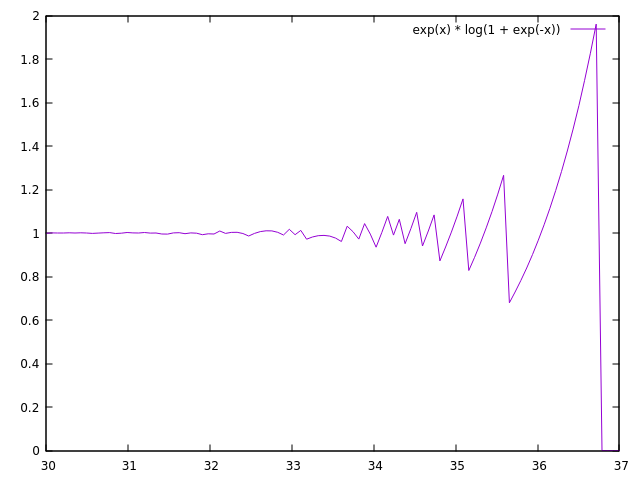
\includegraphics[width=\textwidth]{gnuplot_30_37.png}                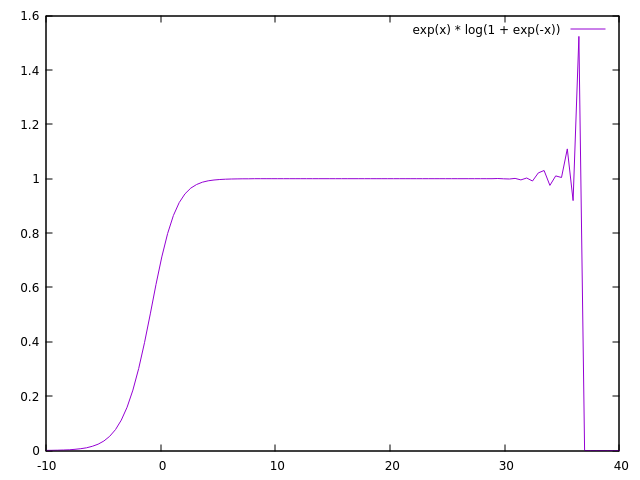
\includegraphics[width=\textwidth]{gnuplot_-10_40.png}
                \caption{Wykresy wygenerowane przy pomocy GNUPLOT}
                \label{fig:gnuplot}
            \end{figure}
            \begin{figure}
                \centering                 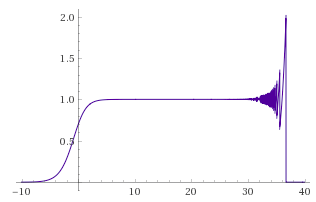
\includegraphics[width=\textwidth]{wolfram_-10_40.png}
                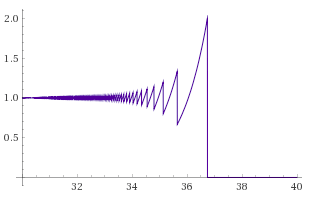
\includegraphics[width=\textwidth]{wolfram_30_40.png}
                \caption{Wykresy wygenerowane przy pomocy WOLFRAM ALPHA}
                \label{fig:wolfram}
            \end{figure}
    \section{Rozwiązywanie układu równań liniowych}
        \subsection{Problem}
            Rozważamy rozwiązanie układu równań $Ax = b$, dla danej macierzy współczynników $A \in \mathbb{R}^{n\times n}$ i wektora prawych stron $b\in \mathbb{R}^{n}$. \\
            Macierz $A$ generujemy w następujący sposób:
            \begin{enumerate}
                \item $A = H_n$, gdzie $H_n$ jest macierzą Hilberta stopnia n wygenerowaną za pomocą
funkcji $A=hilb(n)$
                \item $A = R_n$, gdzie $R_n$ jest losową macierzą stopnia n z zadanym wskaźnikiem uwarunkowania
c wygenerowaną za pomocą funkcji $A=matcond(n,c)$
            \end{enumerate}
            Musimy rozwiązać $Ax = b$ za pomocą dwóch algorytmów: eliminacji Gaussa oraz $x = A^{-1}b$.
            Wykonujemy eksperymenty dla macierzy Hilberta $H_n$ z rosnącym stopniem $n > 1$ oraz dla macierzy losowej $R_n$, $n = 5,10,20$ z rosnącym wskaźnikiem uwarunkowania $c = 1,10,10^3,10^7,10^{12},10^{16}$ i obliczamy błędy względne obu metod.
        \subsection{Rozwiązanie}
            Napisano program wykonujący powyższe wymagania, który oblicza dla macierzy Hilberta jak i dla macierzy losowej takie wartości jak: błąd względny metody Gaussa, błąd względny metody odwrotności macierzy, wskaźnik uwarunkowania badanej macierzy oraz jej rząd. Implementacja w języku \texttt{Julia}.
        \subsection{Wyniki}
            Uzyskano następujące wyniki, pokazane w tabelach \ref{table:zad3:hilbert} oraz \ref{table:zad3:random}.
            {\small
            \begin{table}[h!]
            \begin{tabular}{l l l l l}
                \hline
                 n & Gauss & Inv & Cond & Rank \\
                 \hline
                1 & 0.0 & 0.0 & 1.0 & 1 \\
2 & 5.661048867003676e-16 & 1.4043333874306803e-15 & 19.28147006790397 & 2 \\
3 & 8.022593772267726e-15 & 0.0 & 524.0567775860644 & 3 \\
4 & 4.137409622430382e-14 & 0.0 & 15513.73873892924 & 4 \\
5 & 1.6828426299227195e-12 & 3.3544360584359632e-12 & 476607.25024259434 & 5 \\
6 & 2.618913302311624e-10 & 2.0163759404347654e-10 & 1.4951058642254665e7 & 6 \\
7 & 1.2606867224171548e-8 & 4.713280397232037e-9 & 4.75367356583129e8 & 7 \\
8 & 6.124089555723088e-8 & 3.07748390309622e-7 & 1.5257575538060041e10 & 8 \\
9 & 3.8751634185032475e-6 & 4.541268303176643e-6 & 4.931537564468762e11 & 9 \\
10 & 8.67039023709691e-5 & 0.0002501493411824886 & 1.6024416992541715e13 & 10 \\
11 & 0.00015827808158590435 & 0.007618304284315809 & 5.222677939280335e14 & 11 \\
12 & 0.13396208372085344 & 0.258994120804705 & 1.7514731907091464e16 & 11 \\
13 & 0.11039701117868264 & 5.331275639426837 & 3.344143497338461e18 & 11 \\
14 & 1.4554087127659643 & 8.71499275104814 & 6.200786263161444e17 & 12 \\
15 & 4.696668350857427 & 7.344641453111494 & 3.674392953467974e17 & 12 \\
16 & 54.15518954564602 & 29.84884207073541 & 7.865467778431645e17 & 12 \\
17 & 13.707236683836307 & 10.516942378369349 & 1.263684342666052e18 & 12 \\
18 & 9.134134521198485 & 7.575475905055309 & 2.2446309929189128e18 & 12 \\
                \hline
            \end{tabular}
            \caption{Błędy, wskaźnik uwarunkowania i rząd dla macierzy Hilberta}
            \label{table:zad3:hilbert}
            \end{table}
            }
            
            {\small
            \begin{table}[h!]
            \begin{tabular}{l l l l l l}
                \hline
                 n & c & Gauss & Inv & Cond & Rank \\
                 \hline
5 & 1.0 & 1.719950113979703e-16 & 1.7901808365247238e-16 & 1.0000000000000009 & 5 \\
5 & 10.0 & 2.381163109968744e-16 & 1.9229626863835638e-16 & 10.000000000000004 & 5 \\
5 & 1000.0 & 1.4649896587576702e-14 & 9.532931148469528e-15 & 1000.0000000000565 & 5 \\
5 & 1.0e7 & 2.545190235354581e-10 & 2.4369570680331473e-10 & 9.999999997294577e6 & 5 \\
5 & 1.0e12 & 3.416049679263684e-5 & 3.343033187897742e-5 & 1.0000484354173798e12 & 5 \\
5 & 1.0e16 & 0.0982032383014505 & 0.14925760292611562 & 5.045253102924761e15 & 4 \\
10 & 1.0 & 2.1355566272775288e-16 & 2.830524433501838e-16 & 1.0000000000000009 & 10 \\
10 & 10.0 & 1.890641683868921e-16 & 3.3121136700345433e-16 & 9.999999999999995 & 10 \\
10 & 1000.0 & 1.454667573192289e-14 & 1.6227192306827873e-14 & 999.9999999999449 & 10 \\
10 & 1.0e7 & 2.938368557913579e-10 & 3.246088394336096e-10 & 9.999999994371504e6 & 10 \\
10 & 1.0e12 & 4.491533894867606e-5 & 4.1020191951648577e-5 & 9.999916725791464e11 & 10 \\
10 & 1.0e16 & 0.9335544430733206 & 0.8946182408575178 & 1.4638406408363638e16 & 9 \\
20 & 1.0 & 5.183683495748049e-16 & 4.406061034464155e-16 & 1.0000000000000018 & 20 \\
20 & 10.0 & 3.789423922623494e-16 & 3.8298671591131183e-16 & 10.000000000000007 & 20 \\
20 & 1000.0 & 1.3188496276310147e-14 & 1.608559532353378e-14 & 1000.0000000000059 & 20 \\
20 & 1.0e7 & 7.334798281596067e-11 & 8.86801641837911e-11 & 9.99999999819007e6 & 20 \\
20 & 1.0e12 & 1.7902073255017923e-6 & 5.272232148050303e-6 & 9.999513645109017e11 & 20 \\
20 & 1.0e16 & 0.1359985709340461 & 0.0606916112793811 & 6.764850422530947e15 & 19 \\
                \hline
            \end{tabular}
            \caption{Błędy, wskaźnik uwarunkowania i rząd dla macierzy losowej}
            \label{table:zad3:random}
            \end{table}
            }
        \subsection{Wnioski}
            Błąd względny dla macierzy Hilberta rośnie razem ze zwiększającym się uwarunkowaniem macierzy, co w przypadku macierzy Hilberta jest jednoznacznie związane z jej wielkością. Obserwujemy sumarycznie większy błąd względny gdy do obliczeń używana jest metoda inwersji. W przypadku macierzy generowanej losowo, bezpośredni wpływ na błąd obliczeń ma stopień macierzy i oraz jej wskaźnik uwarunkowania. Im wskaźnik jest większy, tym większe otrzymamy odchylenia od oczekiwanego wyniku.
            
    \section{Wilkinson}
        \subsection{Problem}
            Badamy "złośliwy wielomian Wilkinsona", postaci
            \begin{center}
                $p(x) = \prod_{i=1}^{20}(x - i)$ \\
                
            \end{center}
            \begin{center}
                $P(x) = x^{20} - 210x^{19} - 20615x^{18} - ...$    
            \end{center}
            Mamy sprawdzić obliczone pierwiastki $x_k, 1\leq k \leq 20$, obliczając $|P(z_k)|$, $|p(z_k)|$ i $|z_k - k|$.
        \subsection{Rozwiązanie}
            Napisano program w języku \texttt{Julia} wykorzystujący pakiet \texttt{Polynomials}, umożliwiający manipulację wielomianami. Utworzono wielomian $P(x)$ ze zbioru współczynników (współczynniki ilorazu wielomianu $p(x)$) oraz wielomian $p(x)$ z ilorazu $(x - i), i \in [1..20]$.
            Obliczono pierwiastki $z_k, k \in [1..20]$ wielomianu $P(x)$ za pomocą funkcji \texttt{roots()}, a następnie policzono wartości wielomianów od pierwiastków. Następnie eksperyment powtórzono, zmieniając drugi współczynnik z $-210$ na $-210-2^{-23}$.
        \subsubsection{Wyniki}
            Wyniki przedstawiają tabele \ref{table:zad4:before} oraz \ref{table:zad4:after}
            {\small
            \begin{table}[h!]
            \begin{tabular}{l l l l l}
                \hline
                 k & $z_k$ & $|P(z_k)|$ & |$p(z_k)|$ & $|z_k - k|$ \\
                 \hline
1 & 19.999809291236637 & 2.7462952745472e13 & 1.4019117414364248e23 & 0.00019070876336257925 \\
2 & 19.00190981829944 & 1.0278376162816e13 & 1.1990376202486947e23 & 0.0019098182994383706 \\
3 & 17.99092135271648 & 7.199554861056e12 & 1.0144799361089491e23 & 0.009078647283519814 \\
4 & 17.025427146237412 & 3.777623778304e12 & 8.568905825727875e22 & 0.025427146237412046 \\
5 & 15.946286716607972 & 1.555027751936e12 & 7.01087410689741e22 & 0.05371328339202819 \\
6 & 15.075493799699476 & 6.13987753472e11 & 5.901011420239329e22 & 0.07549379969947623 \\
7 & 13.914755591802127 & 3.65383250944e11 & 4.612719853149547e22 & 0.08524440819787316 \\
8 & 13.07431403244734 & 2.15723629056e11 & 3.807325552825022e22 & 0.07431403244734014 \\
9 & 11.953283253846857 & 7.216771584e10 & 2.8869446884129956e22 & 0.04671674615314281 \\
10 & 11.025022932909318 & 3.5759895552e10 & 2.2478332979247994e22 & 0.025022932909317674 \\
11 & 9.990413042481725 & 1.2707126784e10 & 1.6552601335207813e22 & 0.009586957518274986 \\
12 & 9.002915294362053 & 4.465326592e9 & 1.196559421646318e22 & 0.002915294362052734 \\
13 & 7.999355829607762 & 1.682691072e9 & 8.26205014011023e21 & 0.0006441703922384079 \\
14 & 7.000102002793008 & 4.80398336e8 & 5.423593016891272e21 & 0.00010200279300764947 \\
15 & 5.999989245824773 & 1.20152064e8 & 3.320394888870126e21 & 1.0754175226779239e-5 \\
16 & 5.000000665769791 & 2.4114688e7 & 1.8446752056545675e21 & 6.657697912970661e-7 \\
17 & 3.9999999837375317 & 3.106816e6 & 8.854437035384718e20 & 1.626246826091915e-8 \\
18 & 2.9999999995920965 & 209408.0 & 3.320413931687578e20 & 4.0790348876384996e-10 \\
19 & 2.0000000000283182 & 181760.0 & 7.378697629901744e19 & 2.8318236644508943e-11 \\
20 & 0.9999999999996989 & 36352.0 & 5.517824e6 & 3.0109248427834245e-13 \\
                \hline
            \end{tabular}
            \caption{Wyniki wielomianu Wilkinsona od obliczonego pierwiastka}
            \label{table:zad4:before}
            \end{table}
            }
            
            {\small
            \begin{table}[h!]
            \begin{tabular}{l l l l l}
                \hline
                 k & $z_k$ & $|P(z_k)|$ & |$p(z_k)|$ & $|z_k - k|$ \\
                 \hline
        1 & 20.846910 + 0.0im & 1.114453504512e13 & 1.591108408283123e23 & 0.8469102151947894 \\
        2 & 19.502442 + 1.940331im & 9.539424609817828e12 & 1.318194782057474e23 & 2.004329444309949 \\
        3 & 19.502442 - 1.940331im & 9.539424609817828e12 & 1.318194782057474e23 & 2.454021446312976 \\
        4 & 16.730744 + 2.812624im & 3.315103475981763e11 & 8.484694713574187e22 & 2.825483521349608 \\
        5 & 16.730744 - 2.812624im & 3.315103475981763e11 & 8.484694713574187e22 & 2.9060018735375106 \\
        6 & 13.992406 + 2.518824im & 1.0612064533081976e11 & 4.934647147685479e22 & 2.7128805312847097 \\
        7 & 13.992406 - 2.518824im & 1.0612064533081976e11 & 4.934647147685479e22 & 2.5188358711909045 \\
        8 & 11.793890 + 1.652477im & 3.357756113171857e10 & 2.8568401004080516e22 & 2.045820276678428 \\
        9 & 11.793890 - 1.652477im & 3.357756113171857e10 & 2.8568401004080516e22 & 1.665281290598479 \\
        10 & 10.09545 + 0.644932im & 7.143113638035824e9 & 1.7212892853671066e22 & 1.1109180272716561 \\
        11 & 10.09545 - 0.644932im & 7.143113638035824e9 & 1.7212892853671066e22 & 0.6519586830380406 \\
        12 & 8.915816 + 0.0im & 3.065575424e9 & 1.1607472501770085e22 & 0.0841836320674414 \\
        13 & 8.007772 + 0.0im & 1.072547328e9 & 8.289399860984229e21 & 0.007772029099445632 \\
        14 & 6.999602 + 0.0im & 3.88123136e8 & 5.422366528916045e21 & 0.00039792957757978087 \\
        15 & 6.000020 + 0.0im & 1.29148416e8 & 3.320450195282314e21 & 2.0476673030955794e-5 \\
        16 & 4.999998 + 0.0im & 3.9463936e7 & 1.8446726974084148e21 & 1.4261120897529622e-6 \\
        17 & 4.000000 + 0.0im & 1.046784e7 & 8.854437817429645e20 & 8.972436216225788e-8 \\
        18 & 2.999999 + 0.0im & 2.221568e6 & 3.3204139201100146e20 & 3.3965799062229962e-9 \\
        19 & 2.000000 + 0.0im & 349184.0 & 7.37869763029606e19 & 5.503730804434781e-11 \\
        20 & 0.999999 + 0.0im & 20992.0 & 3.012096e6 & 1.6431300764452317e-13 \\
                \hline
            \end{tabular}
            \caption{Wyniki wielomianu Wilkinsona od obliczonego pierwiastka, ze zmodyfikowanym współczynnikiem $-210$ na $-210-2^{-23}$}
            \label{table:zad4:after}
            \end{table}
            }
        \subsection{Wnioski}
            Mogliśmy się spodziewać, że wyniki obu funkcji będą równe zeru, jeśli wywołamy je z argumentem równym pierwiastkowi wielomianu. Tak jednak nie jest, a wyniki są bardzo dalekie od zera. Błąd obliczeń, który bierze się z niedokładności przedstawienia współczynników wielomianu buduje błąd, który narasta wraz z każdą kolejną operacją. Współczynniki wielomianu $P(x)$ są reprezentowane z błędem, ponieważ w arytmetyce \texttt{Float64} mamy około 15 do 17 miejsc na cyfry znaczące systemu dziesiętnego. \\
            Następny eksperyment, w którym zmieniliśmy współczynnik przy $x^{19}$ spowodował, że miejsca zerowe stały się liczbami zespolonymi. Ta minimalna zmiana sprawiła, że wyniki zmieniły się diametralnie. Zadanie jest więc źle uwarunkowane.
        
    \section{Model wzrostu populacji}
        \subsection{Problem}
            Przeprowadzić eksperymenty wykorzystując następujący model:
            \begin{center}
                $p_{n+1} := p_n + rp_{n}(1 - p_n)$, dla $n = 0, 1, . . . ,$ \\
                $p_0 = 0.01, r = 3$
            \end{center}
            \begin{enumerate}
                \item Wykonać 40 iteracji powyższego wyrażenia w arytmetyce Float32
                \item Wykonać 40 iteracji, ale po 10 iteracji obciąć wynik do 3 miejsc po przecinku i kontynuować do 40 iteracji w arytmetyce Float32
                \item Wykonać 40 iteracji w arytmetyce Float64
            \end{enumerate}
        \subsection{Rozwiązanie}
            Zaimplementowano funkcję realizującą w sposób iteracyjny powyższy wzór rekurencyjny, z parametrem pozwalającym obciąć wynik 10-tej iteracji do trzech miejsc po przecinku. Funkcja jest inicjalizowana $p_n = p_0$, a w kolejnych iteracjach wartość $p_n$ zastępowana jest przez $p_n + r \cdot pn \cdot (1 - p_n)$, dopóki, dopóty nie osiągniemy żądanego $n$. Program został zaimplementowany w języku \texttt{Julia}.
        \subsection{Wyniki}
            Wyniki zostały przedstawione w tabeli \ref{table:zad5}
            {\small
            \begin{table}[h!]
            \begin{tabular}{l l l l}
                \hline
                 i & Float32 + Obciecie & Float32 & Float64 \\
                 \hline
        1 & 0.0397 & 0.0397 & 0.0397 \\
2 & 0.15407173 & 0.15407173 & 0.15407173000000002 \\
3 & 0.5450726 & 0.5450726 & 0.5450726260444213 \\
4 & 1.2889781 & 1.2889781 & 1.2889780011888006 \\
5 & 0.1715188 & 0.1715188 & 0.17151914210917552 \\
6 & 0.5978191 & 0.5978191 & 0.5978201201070994 \\
7 & 1.3191134 & 1.3191134 & 1.3191137924137974 \\
8 & 0.056273222 & 0.056273222 & 0.056271577646256565 \\
9 & 0.21559286 & 0.21559286 & 0.21558683923263022 \\
10 & 0.722 & 0.7229306 & 0.722914301179573 \\
11 & 1.3241479 & 1.3238364 & 1.3238419441684408 \\
12 & 0.036488414 & 0.037716985 & 0.03769529725473175 \\
13 & 0.14195944 & 0.14660022 & 0.14651838271355924 \\
14 & 0.50738037 & 0.521926 & 0.521670621435246 \\
15 & 1.2572169 & 1.2704837 & 1.2702617739350768 \\
16 & 0.28708452 & 0.2395482 & 0.24035217277824272 \\
17 & 0.9010855 & 0.7860428 & 0.7881011902353041 \\
18 & 1.1684768 & 1.2905813 & 1.2890943027903075 \\
19 & 0.577893 & 0.16552472 & 0.17108484670194324 \\
20 & 1.3096911 & 0.5799036 & 0.5965293124946907 \\
21 & 0.09289217 & 1.3107498 & 1.3185755879825978 \\
22 & 0.34568182 & 0.088804245 & 0.058377608259430724 \\
23 & 1.0242395 & 0.3315584 & 0.22328659759944824 \\
24 & 0.94975823 & 0.9964407 & 0.7435756763951792 \\
25 & 1.0929108 & 1.0070806 & 1.315588346001072 \\
26 & 0.7882812 & 0.9856885 & 0.07003529560277899 \\
27 & 1.2889631 & 1.0280086 & 0.26542635452061003 \\
28 & 0.17157483 & 0.9416294 & 0.8503519690601384 \\
29 & 0.59798557 & 1.1065198 & 1.2321124623871897 \\
30 & 1.3191822 & 0.7529209 & 0.37414648963928676 \\
31 & 0.05600393 & 1.3110139 & 1.0766291714289444 \\
32 & 0.21460639 & 0.0877831 & 0.8291255674004515 \\
33 & 0.7202578 & 0.3280148 & 1.2541546500504441 \\
34 & 1.3247173 & 0.9892781 & 0.29790694147232066 \\
35 & 0.034241438 & 1.021099 & 0.9253821285571046 \\
36 & 0.13344833 & 0.95646656 & 1.1325322626697856 \\
37 & 0.48036796 & 1.0813814 & 0.6822410727153098 \\
38 & 1.2292118 & 0.81736827 & 1.3326056469620293 \\
39 & 0.3839622 & 1.2652004 & 0.0029091569028512065 \\
40 & 1.093568 & 0.25860548 & 0.011611238029748606 \\
                \hline
            \end{tabular}
            \caption{Kolejne iteracje funkcji wzrostu populacji}
            \label{table:zad5}
            \end{table}
            }
        \subsection{Wnioski}
            Pierwszym spostrzeżeniem jest, że wyniki końcowe, różnią się dla każdego eksperymentu. Pierwsze kilka wyników jest takie samo dla każdego z eksperymentów, natomiast błąd narastający z powodu ograniczonej precyzji arytmetyki prowadzi do niewiarygodnych wyników. Można zauważyć, że dla eksperymentów w arytmetyce \texttt{Float32}, rozbieżności zaczynają się bardzo szybko. Jeszcze szybciej dzieje się to w przypadku gdy dojdzie do obcięcia do trzech miejsc po przecinku dziesiątej operacji. \texttt{Float64} radzi sobie nieco lepiej, ale ze względów na kwadratowy wzrost wartości tracimy cyfry znaczące i nawet podwójna precyzja w niczym tu nie pomaga. Nie jesteśmy w stanie stwierdzić, który eksperyment dał prawidłowe wyniki - możemy jedynie przypuszczać, że był to \texttt{Float64} (a przynajmniej, do pewnego $n$). Ten typ zależności rekurencyjnej nazywamy sprzężeniem zwrotnym, w którym wynik jest używany jako wejście (np. do procesora) i ponownie przetwarzany. W sprzężeniu zwrotnym, lekkie zaburzenie początkowych obliczeń ma olbrzymi wpływ na wynik końcowy, więc to zadanie nie jest dobrze uwarunkowane.
        
    \section{Równanie rekurencyjne}
        \subsection{Problem}
            Rozważamy równanie rekurencyjne
            \begin{center}
                $x_{n+1} := x_{n}^2 + c$ dla $n = 0, 1, ...$
            \end{center}
            W arytmetyce \texttt{Float64} wykonujamy 40 iteracji dla danych:
            \begin{enumerate}
                \item $c = -2$ i $z_0 = 1$
                \item $c = -2$ i $z_0 = 2$
                \item $c = -2$ i $z_0 = 1.99999999999999$
                \item $c = -1$ i $z_0 = 1$
                \item $c = -1$ i $z_0 = -1$
                \item $c = -1$ i $z_0 = 0.75$
                \item $c = -1$ i $z_0 = 0.25$
            \end{enumerate}
        \subsection{Rozwiązanie}
            Napisano program obliczający powyższą zależność rekurencyjną, dla każdego $i \in [1..40]$ i dla każdej pary $(c, x_0)$. Na podstawie tych siedmiu zbiorów danych generujemy wykresy funkcji reprezentujące wyniki.
        \subsection{Wyniki}
            Wyniki zostały przedstawione na wykresach (rysunkach)
            \ref{fig:zad6:fig1},
            \ref{fig:zad6:fig2},
            \ref{fig:zad6:fig3} oraz
            \ref{fig:zad6:fig4}
            \begin{figure}
                \centering                 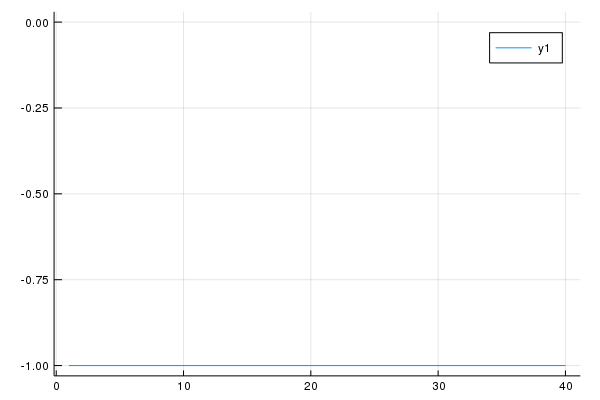
\includegraphics[width=0.49\linewidth]{plot_1.png}                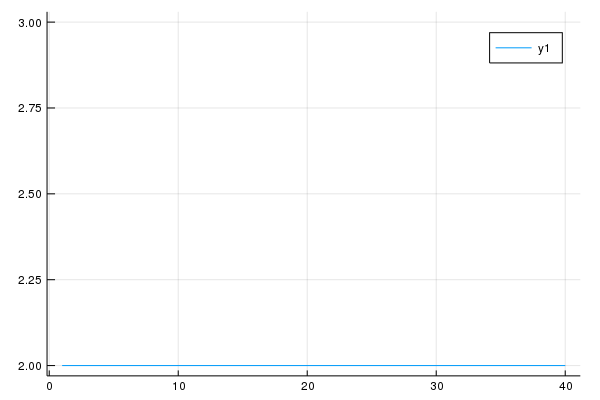
\includegraphics[width=0.49\linewidth]{plot_2.png}
                \caption{$c = -2, x_0 = 1$ oraz $c = -2, x_0 = 2$}
                \label{fig:zad6:fig1}
            \end{figure}
            \begin{figure}
                \centering                 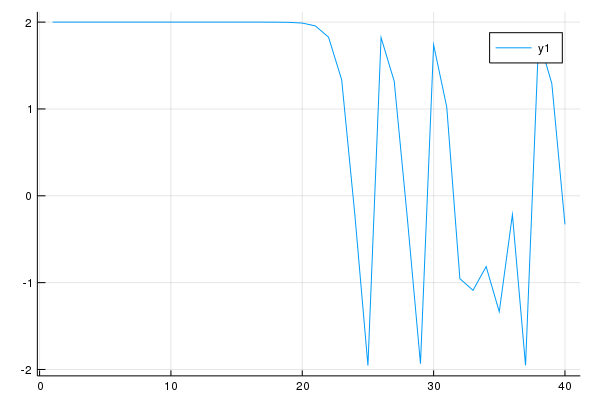
\includegraphics[width=0.49\linewidth]{plot_3.png}                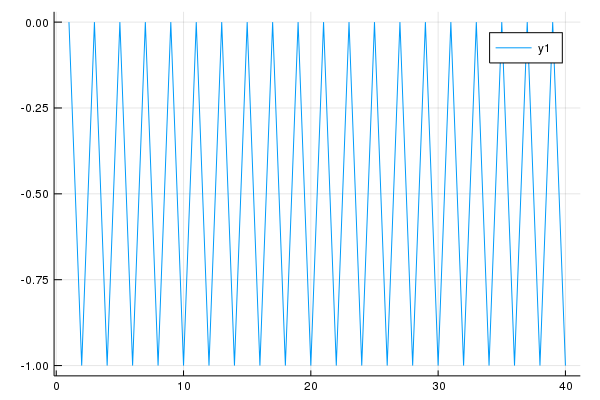
\includegraphics[width=0.49\linewidth]{plot_4.png}
                \caption{$c = -2, x_0 = 1.99999999999999$ oraz $c = -1, x_0 = 1$}
                \label{fig:zad6:fig2}
            \end{figure}
            \begin{figure}
                \centering                 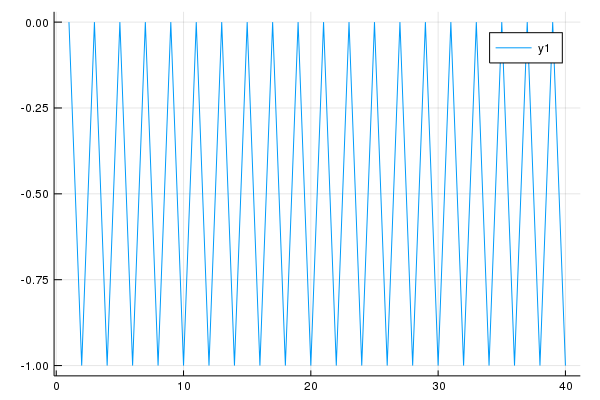
\includegraphics[width=0.49\linewidth]{plot_5.png}                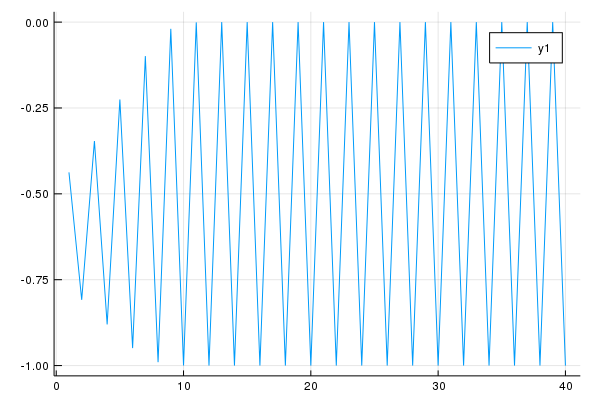
\includegraphics[width=0.49\linewidth]{plot_6.png}
                \caption{$c = -1, x_0 = -1$ oraz $c = -1, x_0 = 0.75$}
                \label{fig:zad6:fig3}
            \end{figure}
            \begin{figure}
                \centering                 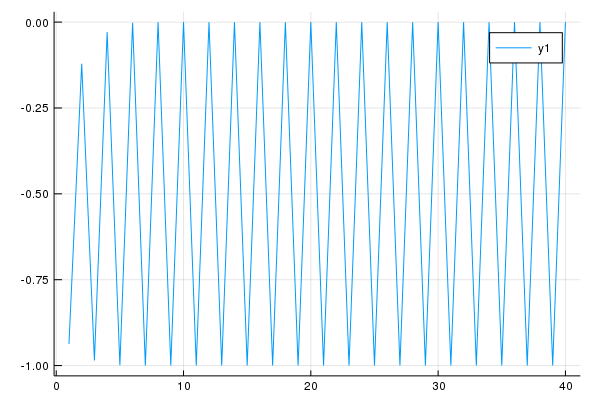
\includegraphics[width=\linewidth]{plot_7.png}
                \caption{$c = -1, x_0 = -1$ oraz $c = -1, x_0 = 0.25$}
                \label{fig:zad6:fig4}
            \end{figure}
        \subsection{Wnioski}
            Wspomagając się literaturą "Granice Chaosu" i analizując badaną funkcję za pomocą metody iteracji graficznej jak i również wykresów oraz wyników programu będziemy rozważać okresowość wyników. Dla niektórych danych obserwujemy wartości zbieżne idealnie, to znaczy przyjmujących stałą wartość lub wartości dla każdego z wyników. Kolejnym typem są ciągi zbieżne do danej liczby, gdy ${n\rightarrow \infty}$, gdzie n to liczba iteracji. Istnieje jeszcze klasa ciągów rozbieżnych, które przy metodzie iteracji graficznej będą dążyły do zakreślenia całej powierzchni wykresu i nigdy nie zbiegną (lub posiadają zbyt duży okres) jak zobaczylibyśmy dla przykładu $(c = -2, x_0 = 1.99999999999999)$ gdy $n\rightarrow \infty$.
\end{document}
